\documentclass{article}
\usepackage{amsmath}
\usepackage{geometry}
\usepackage{fancyhdr}
\usepackage{lipsum}
\usepackage{enumitem}
\usepackage{amsfonts}
\usepackage{graphicx}
\usepackage{pgfplots}
\pgfplotsset{compat=1.18}

\geometry{margin=1in}
\pagestyle{fancy}
\fancyhf{}
\fancyhead[L]{Mathematical and Numerical Methods for Biologists}
\fancyhead[R]{BB 523}
\fancyfoot[C]{\thepage}

\title{Practice Questions in Differentiation Solutions}
\author{}
\date{\today}

\begin{document}

\maketitle
\thispagestyle{fancy}



\begin{enumerate}[itemsep=20pt]

    \item \textbf{Solution to Question 1:}
    \begin{enumerate}[label=(\alph*), itemsep=10pt]
        \item The gradient vector \( \nabla f(x, y) \) is given by:
        \[
        \nabla f(x, y) = \left( \frac{\partial f}{\partial x}, \frac{\partial f}{\partial y} \right)
        \]
        For the function \( f(x, y) = 3x^2 + 4xy + 2y^2 \), we calculate the partial derivatives:
        \[
        \frac{\partial f}{\partial x} = 6x + 4y, \quad \frac{\partial f}{\partial y} = 4x + 4y
        \]
        Therefore, at the point \( (1, 2) \):
        \[
        \nabla f(1, 2) = \left( 6(1) + 4(2), 4(1) + 4(2) \right) = \left( 6 + 8, 4 + 8 \right) = (14, 12)
        \]
        
        \item The gradient vector \( \nabla f(1, 2) = (14, 12) \) points in the direction of the steepest ascent. This means that at the point \( (1, 2) \), the function increases most rapidly in the direction of the vector \( (14, 12) \).
    \end{enumerate}

    \item \textbf{Solution to Question 2:}
    The derivative of a function \( h(x) \) at a point \( x = a \) using the limit definition is given by:
\[
h'(a) = \lim_{h \to 0} \frac{h(a+h) - h(a)}{h}
\]
For the function \( h(x) = \sqrt{x} \) at \( x = 4 \), we have:
\[
h'(4) = \lim_{h \to 0} \frac{\sqrt{4+h} - \sqrt{4}}{h}
\]
Simplify the expression:
\[
h'(4) = \lim_{h \to 0} \frac{\sqrt{4+h} - 2}{h}
\]
To evaluate this limit, multiply the numerator and the denominator by the conjugate of the numerator:
\[
h'(4) = \lim_{h \to 0} \frac{(\sqrt{4+h} - 2)(\sqrt{4+h} + 2)}{h(\sqrt{4+h} + 2)}
\]
This simplifies to:
\[
h'(4) = \lim_{h \to 0} \frac{4 + h - 4}{h(\sqrt{4+h} + 2)} = \lim_{h \to 0} \frac{h}{h(\sqrt{4+h} + 2)}
\]
Cancel out the \( h \) terms:
\[
h'(4) = \lim_{h \to 0} \frac{1}{\sqrt{4+h} + 2}
\]
As \( h \) approaches 0, \( \sqrt{4+h} \) approaches \( \sqrt{4} = 2 \):
\[
h'(4) = \frac{1}{2 + 2} = \frac{1}{4}
\]
Thus, the derivative of \( h(x) = \sqrt{x} \) at \( x = 4 \) is:
\[
h'(4) = \frac{1}{4}
\]

    \item \textbf{Solution to Question 3:}
    \subsection*{(a) \( f(x) = x^3 \)}

The derivative of \( f(x) \) using the limit definition is:
\[
f'(x) = \lim_{h \to 0} \frac{f(x+h) - f(x)}{h}
\]
Substituting \( f(x) = x^3 \):
\[
f'(x) = \lim_{h \to 0} \frac{(x+h)^3 - x^3}{h}
\]
Expanding \( (x+h)^3 \) using the binomial theorem:
\[
(x+h)^3 = x^3 + 3x^2h + 3xh^2 + h^3
\]
So,
\[
f'(x) = \lim_{h \to 0} \frac{x^3 + 3x^2h + 3xh^2 + h^3 - x^3}{h} = \lim_{h \to 0} \frac{3x^2h + 3xh^2 + h^3}{h}
\]
Factor out \( h \) from the numerator:
\[
f'(x) = \lim_{h \to 0} \left(3x^2 + 3xh + h^2\right)
\]
As \( h \) approaches 0:
\[
f'(x) = 3x^2
\]
\subsection*{(b) \( F(x) = x^2 \)}
Using the limit definition:
\[
F'(x) = \lim_{h \to 0} \frac{(x+h)^2 - x^2}{h}
\]
Expanding \( (x+h)^2 \):
\[
(x+h)^2 = x^2 + 2xh + h^2
\]
So,
\[
F'(x) = \lim_{h \to 0} \frac{x^2 + 2xh + h^2 - x^2}{h} = \lim_{h \to 0} \frac{2xh + h^2}{h}
\]
Simplifying:
\[
F'(x) = \lim_{h \to 0} \left(2x + h\right)
\]
As \( h \) approaches 0:
\[
F'(x) = 2x
\]

\subsection*{(c) \( f(x) = 2x + 3 \)}

Using the limit definition:
\[
f'(x) = \lim_{h \to 0} \frac{f(x+h) - f(x)}{h}
\]
Substituting \( f(x) = 2x + 3 \):
\[
f'(x) = \lim_{h \to 0} \frac{(2(x+h) + 3) - (2x + 3)}{h} = \lim_{h \to 0} \frac{2x + 2h + 3 - 2x - 3}{h}
\]
Simplifying:
\[
f'(x) = \lim_{h \to 0} \frac{2h}{h} = \lim_{h \to 0} 2 = 2
\]
So, the derivative is:
\[
f'(x) = 2
\]

\subsection*{(d) \( f(x) = 5x - 7 \)}

Using the limit definition:
\[
f'(x) = \lim_{h \to 0} \frac{f(x+h) - f(x)}{h}
\]
Substituting \( f(x) = 5x - 7 \):
\[
f'(x) = \lim_{h \to 0} \frac{5(x+h) - 7 - (5x - 7)}{h} = \lim_{h \to 0} \frac{5x + 5h - 7 - 5x + 7}{h}
\]
Simplifying:
\[
f'(x) = \lim_{h \to 0} \frac{5h}{h} = \lim_{h \to 0} 5 = 5
\]
So, the derivative is:
\[
f'(x) = 5
\]

\subsection*{(e) \( f(x) = x^3 - 2x^2 + x - 8 \)}

Using the limit definition:
\[
f'(x) = \lim_{h \to 0} \frac{f(x+h) - f(x)}{h}
\]
Substituting \( f(x) = x^3 - 2x^2 + x - 8 \):
\[
f'(x) = \lim_{h \to 0} \frac{(x+h)^3 - 2(x+h)^2 + (x+h) - 8 - \left( x^3 - 2x^2 + x - 8 \right)}{h}
\]
Expanding \( (x+h)^3 \) and \( (x+h)^2 \):
\[
(x+h)^3 = x^3 + 3x^2h + 3xh^2 + h^3
\]
\[
(x+h)^2 = x^2 + 2xh + h^2
\]
So,
\[
f'(x) = \lim_{h \to 0} \frac{x^3 + 3x^2h + 3xh^2 + h^3 - 2(x^2 + 2xh + h^2) + x + h - 8 - x^3 + 2x^2 - x + 8}{h}
\]
Simplifying:
\[
f'(x) = \lim_{h \to 0} \frac{3x^2h + 3xh^2 + h^3 - 2x^2 - 4xh - 2h^2 + h}{h} = \lim_{h \to 0} \frac{(3x^2 - 4x + 1)h + (3xh^2 - 2h^2 + h^3)}{h}
\]
Simplifying further:
\[
f'(x) = \lim_{h \to 0} \left(3x^2 - 4x + 1 + h(3x - 2 + h)\right)
\]
As \( h \) approaches 0:
\[
f'(x) = 3x^2 - 4x + 1
\]
    \end{enumerate}
    
   \item \textbf{Solution to Question 4:}
    \begin{enumerate}[label=(\alph*), itemsep=10pt]
    \item The function is given by \( f(x) = x^3 - 6x^2 + 9x + 1 \). To find the local minima and maxima, we first compute the first derivative:
    \[
    f'(x) = \frac{d}{dx}(x^3 - 6x^2 + 9x + 1) = 3x^2 - 12x + 9
    \]
    
    \item To find the critical points, we set the first derivative equal to zero:
    \[
    3x^2 - 12x + 9 = 0
    \]
    Divide through by 3:
    \[
    x^2 - 4x + 3 = 0
    \]
    Factor the quadratic equation:
    \[
    (x - 1)(x - 3) = 0
    \]
    Therefore, the critical points are:
    \[
    x = 1 \quad \text{and} \quad x = 3
    \]

    \item Next, we find the second derivative to classify these critical points:
    \[
    f''(x) = \frac{d}{dx}(3x^2 - 12x + 9) = 6x - 12
    \]
    Evaluate \( f''(x) \) at the critical points:
    \begin{itemize}
        \item For \( x = 1 \):
        \[
        f''(1) = 6(1) - 12 = 6 - 12 = -6
        \]
        Since \( f''(1) < 0 \), the function has a local maximum at \( x = 1 \).

        \item For \( x = 3 \):
        \[
        f''(3) = 6(3) - 12 = 18 - 12 = 6
        \]
        Since \( f''(3) > 0 \), the function has a local minimum at \( x = 3 \).
    \end{itemize}

    \item Finally, evaluate the function at the critical points to determine the local minima and maxima:
    \begin{itemize}
        \item At \( x = 1 \):
        \[
        f(1) = 1^3 - 6(1)^2 + 9(1) + 1 = 1 - 6 + 9 + 1 = 5
        \]
        Thus, there is a local maximum at \( (1, 5) \).

        \item At \( x = 3 \):
        \[
        f(3) = 3^3 - 6(3)^2 + 9(3) + 1 = 27 - 54 + 27 + 1 = 1
        \]
        Thus, there is a local minimum at \( (3, 1) \).
    \end{itemize}
\end{enumerate}
    \item \textbf{Solution to Question 5:}
\begin{enumerate}[label=(\alph*), itemsep=10pt]
    \item The function is given by \( f(x) = x^4 - 4x^3 + 4x^2 \). To find the critical points, we first compute the first derivative:
    \[
    f'(x) = \frac{d}{dx}(x^4 - 4x^3 + 4x^2) = 4x^3 - 12x^2 + 8x
    \]

    \item Set the first derivative equal to zero to find the critical points:
    \[
    4x^3 - 12x^2 + 8x = 0
    \]
    Factor out the common term \( 4x \):
    \[
    4x(x^2 - 3x + 2) = 0
    \]
    Factor the quadratic equation \( x^2 - 3x + 2 \):
    \[
    x^2 - 3x + 2 = (x - 1)(x - 2)
    \]
    Therefore, we have:
    \[
    4x(x - 1)(x - 2) = 0
    \]
    The critical points are:
    \[
    x = 0, \quad x = 1, \quad x = 2
    \]

    \item Next, we find the second derivative to classify these critical points:
    \[
    f''(x) = \frac{d}{dx}(4x^3 - 12x^2 + 8x) = 12x^2 - 24x + 8
    \]

    \item Evaluate \( f''(x) \) at each critical point:
    \begin{itemize}
        \item For \( x = 0 \):
        \[
        f''(0) = 12(0)^2 - 24(0) + 8 = 8
        \]
        Since \( f''(0) > 0 \), there is a local minimum at \( x = 0 \).

        \item For \( x = 1 \):
        \[
        f''(1) = 12(1)^2 - 24(1) + 8 = 12 - 24 + 8 = -4
        \]
        Since \( f''(1) < 0 \), there is a local maximum at \( x = 1 \).

        \item For \( x = 2 \):
        \[
        f''(2) = 12(2)^2 - 24(2) + 8 = 48 - 48 + 8 = 8
        \]
        Since \( f''(2) > 0 \), there is a local minimum at \( x = 2 \).
    \end{itemize}

    \item Finally, evaluate the function at the critical points to determine their nature:
    \begin{itemize}
        \item At \( x = 0 \):
        \[
        f(0) = 0^4 - 4(0)^3 + 4(0)^2 = 0
        \]
        There is a local minimum at \( (0, 0) \).

        \item At \( x = 1 \):
        \[
        f(1) = 1^4 - 4(1)^3 + 4(1)^2 = 1 - 4 + 4 = 1
        \]
        There is a local maximum at \( (1, 1) \).

        \item At \( x = 2 \):
        \[
        f(2) = 2^4 - 4(2)^3 + 4(2)^2 = 16 - 32 + 16 = 0
        \]
        There is a local minimum at \( (2, 0) \).
    \end{itemize}
\end{enumerate}
    \item \textbf{Solution to Question 6:}

To find the points of minima and maxima for \( f(x) = \sin(x) + \cos(x) \) on the interval \([0, 2\pi]\), we first compute the derivative:

\[
f'(x) = \cos(x) - \sin(x)
\]

Setting the derivative equal to zero to find critical points:

\[
\cos(x) - \sin(x) = 0 \implies \cos(x) = \sin(x)
\]

This equality holds when:

\[
x = \frac{\pi}{4} + k\pi \quad \text{for integer } k
\]

Within the interval \([0, 2\pi]\), the critical points are:

\[
x = \frac{\pi}{4}, \frac{5\pi}{4}
\]

To determine whether these points are maxima or minima, we compute the second derivative:

\[
f''(x) = -\sin(x) - \cos(x)
\]

Evaluate \( f''(x) \) at the critical points:

\[
f''\left(\frac{\pi}{4}\right) = -\sin\left(\frac{\pi}{4}\right) - \cos\left(\frac{\pi}{4}\right) = -\sqrt{2}/2 - \sqrt{2}/2 = -\sqrt{2} < 0
\]
Thus, \( x = \frac{\pi}{4} \) is a local maximum.

\[
f''\left(\frac{5\pi}{4}\right) = -\sin\left(\frac{5\pi}{4}\right) - \cos\left(\frac{5\pi}{4}\right) = \sqrt{2}/2 + \sqrt{2}/2 = \sqrt{2} > 0
\]
Thus, \( x = \frac{5\pi}{4} \) is a local minimum.

Evaluate \( f(x) \) at these points:

\[
f\left(\frac{\pi}{4}\right) = \sin\left(\frac{\pi}{4}\right) + \cos\left(\frac{\pi}{4}\right) = \sqrt{2}/2 + \sqrt{2}/2 = \sqrt{2}
\]

\[
f\left(\frac{5\pi}{4}\right) = \sin\left(\frac{5\pi}{4}\right) + \cos\left(\frac{5\pi}{4}\right) = -\sqrt{2}/2 - \sqrt{2}/2 = -\sqrt{2}
\]

Also, evaluate the function at the endpoints:

\[
f(0) = \sin(0) + \cos(0) = 0 + 1 = 1
\]

\[
f(2\pi) = \sin(2\pi) + \cos(2\pi) = 0 + 1 = 1
\]

Therefore, the points of minima and maxima in the interval \([0, 2\pi]\) are:

- Local maximum at \( x = \frac{\pi}{4} \) with \( f\left(\frac{\pi}{4}\right) = \sqrt{2} \)
- Local minimum at \( x = \frac{5\pi}{4} \) with \( f\left(\frac{5\pi}{4}\right) = -\sqrt{2} \)
- Maximum value at endpoints \( x = 0 \) and \( x = 2\pi \) with \( f(0) = 1 \) and \( f(2\pi) = 1 \)
    \item \textbf{Solution to Question 7:}

To find the local extrema of the function \( f(x) = \frac{1}{3}x^3 - 2x^2 + 3x \), we first compute its derivative:

\[
f'(x) = \frac{d}{dx} \left( \frac{1}{3}x^3 - 2x^2 + 3x \right) = x^2 - 4x + 3
\]

Set the derivative equal to zero to find critical points:

\[
x^2 - 4x + 3 = 0
\]

Solve this quadratic equation using factoring:

\[
(x - 1)(x - 3) = 0
\]

Thus, the critical points are:

\[
x = 1 \quad \text{and} \quad x = 3
\]

To determine whether these points are maxima or minima, compute the second derivative:

\[
f''(x) = \frac{d}{dx} (x^2 - 4x + 3) = 2x - 4
\]

Evaluate the second derivative at the critical points:

\[
f''(1) = 2(1) - 4 = -2 \quad (\text{Negative, so } x = 1 \text{ is a local maximum})
\]

\[
f''(3) = 2(3) - 4 = 2 \quad (\text{Positive, so } x = 3 \text{ is a local minimum})
\]

Finally, evaluate \( f(x) \) at the critical points to find the function values:

\[
f(1) = \frac{1}{3}(1)^3 - 2(1)^2 + 3(1) = \frac{1}{3} - 2 + 3 = \frac{4}{3}
\]

\[
f(3) = \frac{1}{3}(3)^3 - 2(3)^2 + 3(3) = \frac{27}{3} - 18 + 9 = 0
\]

Therefore, the local extrema of the function are:

- Local maximum at \( x = 1 \) with \( f(1) = \frac{4}{3} \)
- Local minimum at \( x = 3 \) with \( f(3) = 0 \)
    \item \textbf{Solution to Question 8:}
\begin{enumerate}[label=(\alph*), itemsep=10pt]
    \item To find the minima and maxima of the function \( f(x) = x^2 + \frac{4}{x} \) for \( x > 0 \), we first compute the first derivative:
    \[
    f'(x) = \frac{d}{dx}\left(x^2 + \frac{4}{x}\right) = 2x - \frac{4}{x^2}
    \]

    \item Set the first derivative equal to zero to find the critical points:
    \[
    2x - \frac{4}{x^2} = 0
    \]
    Multiply through by \( x^2 \) to clear the fraction:
    \[
    2x^3 - 4 = 0
    \]
    Solve for \( x \):
    \[
    2x^3 = 4
    \]
    \[
    x^3 = 2
    \]
    \[
    x = \sqrt[3]{2}
    \]

    \item Next, compute the second derivative to classify the critical point:
    \[
    f''(x) = \frac{d}{dx}\left(2x - \frac{4}{x^2}\right) = 2 + \frac{8}{x^3}
    \]

    \item Evaluate \( f''(x) \) at the critical point \( x = \sqrt[3]{2} \):
    \[
    f''\left(\sqrt[3]{2}\right) = 2 + \frac{8}{\left(\sqrt[3]{2}\right)^3}
    \]
    \[
    f''\left(\sqrt[3]{2}\right) = 2 + \frac{8}{2} = 2 + 4 = 6
    \]
    Since \( f''\left(\sqrt[3]{2}\right) > 0 \), the function has a local minimum at \( x = \sqrt[3]{2} \).

    \item Finally, evaluate the function at the critical point to find the minimum value:
    \[
    f\left(\sqrt[3]{2}\right) = \left(\sqrt[3]{2}\right)^2 + \frac{4}{\sqrt[3]{2}}
    \]
    \[
    \left(\sqrt[3]{2}\right)^2 = \sqrt[3]{4}
    \]
    \[
    \frac{4}{\sqrt[3]{2}} = 2 \sqrt[3]{2}
    \]
    \[
    f\left(\sqrt[3]{2}\right) = \sqrt[3]{4} + 2 \sqrt[3]{2}
    \]
    Simplify further:
    \[
    f\left(\sqrt[3]{2}\right) = \sqrt[3]{4} + 2 \cdot \sqrt[3]{2}
    \]
    \[
    f\left(\sqrt[3]{2}\right) = 3 \sqrt[3]{2}
    \]
    So, the local minimum value is \( 3 \sqrt[3]{2} \) at \( x = \sqrt[3]{2} \).

    \item Since the function \( f(x) = x^2 + \frac{4}{x} \) approaches infinity as \( x \to 0^+ \) and \( x \to \infty \), there are no local maxima in the domain \( x > 0 \).
\end{enumerate}
    \item \textbf{Solution to Question 9:}
\begin{enumerate}[label=(\alph*), itemsep=10pt]
    \item To find the extrema of the function \( f(x) = x - \ln(x) \) for \( x > 0 \), we first compute the first derivative:
    \[
    f'(x) = \frac{d}{dx}\left(x - \ln(x)\right) = 1 - \frac{1}{x}
    \]

    \item Set the first derivative equal to zero to find the critical points:
    \[
    1 - \frac{1}{x} = 0
    \]
    Solve for \( x \):
    \[
    \frac{1}{x} = 1
    \]
    \[
    x = 1
    \]

    \item Compute the second derivative to classify the critical point:
    \[
    f''(x) = \frac{d}{dx}\left(1 - \frac{1}{x}\right) = \frac{1}{x^2}
    \]

    \item Evaluate \( f''(x) \) at the critical point \( x = 1 \):
    \[
    f''(1) = \frac{1}{1^2} = 1
    \]
    Since \( f''(1) > 0 \), the function has a local minimum at \( x = 1 \).

    \item Evaluate the function at the critical point to find the minimum value:
    \[
    f(1) = 1 - \ln(1) = 1 - 0 = 1
    \]
    So, the local minimum value is \( 1 \) at \( x = 1 \).

    \item To determine whether there is a maximum, analyze the behavior of \( f(x) \) as \( x \) approaches the boundaries of its domain:
    \begin{itemize}
        \item As \( x \to 0^+ \), \( \ln(x) \to -\infty \) and thus \( f(x) = x - \ln(x) \to \infty \).
        \item As \( x \to \infty \), \( x - \ln(x) \to \infty \) because \( x \) grows faster than \( \ln(x) \).
    \end{itemize}
    Hence, \( f(x) \) does not have a maximum value in the domain \( x > 0 \).

    \item In summary, the function \( f(x) = x - \ln(x) \) has a local minimum value of \( 1 \) at \( x = 1 \) and does not have a maximum value in the domain \( x > 0 \).
\end{enumerate}

    

    \item \textbf{Solution to Question 10:}
    \begin{enumerate}[label=(\alph*), itemsep=10pt]
        \item The population function is \( P(t) = P_0 e^{rt} \). The rate of population growth is given by the derivative with respect to \( t \):
        \[
        \frac{dP}{dt} = P_0 r e^{rt}
        \]
        
        \item The growth rate is maximized when \( \frac{d^2P}{dt^2} = 0 \). Since \( \frac{d^2P}{dt^2} = P_0 r^2 e^{rt} > 0 \) for all \( t \), the growth rate continuously increases, and thus it doesn't have a finite maximum but grows indefinitely as \( t \) increases.
    \end{enumerate}

    \item \textbf{Solution to Question 11:}

    The spread of a disease is modeled by \( I(t) = \frac{1000}{1 + 9e^{-0.5t}} \), where \( I(t) \) is the number of infected individuals at time \( t \).

    \begin{enumerate}[label=(\alph*), itemsep=10pt]
        \item \textbf{Find the rate of change of the number of infected individuals at any time \( t \).}

        The rate of change is found by differentiating \( I(t) \):

        \[
        I'(t) = \frac{d}{dt} \left[ \frac{1000}{1 + 9e^{-0.5t}} \right]
        \]

        Using the chain rule:

        \[
        I'(t) = 1000 \cdot \frac{0.5 \cdot 9e^{-0.5t}}{\left( 1 + 9e^{-0.5t} \right)^2} = \frac{4500e^{-0.5t}}{\left( 1 + 9e^{-0.5t} \right)^2}
        \]

        \item \textbf{Determine the time at which the infection rate is highest.}

        To find the time when the infection rate is highest, set the derivative \( I'(t) \) to zero:

        \[
        \frac{4500e^{-0.5t}}{\left( 1 + 9e^{-0.5t} \right)^2} = 0
        \]

        This expression is never zero for any finite \( t \). Instead, to maximize \( I'(t) \), we observe that \( I'(t) \) increases when \( e^{-0.5t} \) is large and decreases as \( e^{-0.5t} \) becomes small. The infection rate is highest when \( t = 0 \), and it decreases as \( t \) increases.
    \end{enumerate}

    \item \textbf{Solution to Question 12:}
    \begin{enumerate}[label=(\alph*), itemsep=10pt]
        \item The rate of an enzyme-catalyzed reaction is given by \( v(S) = \frac{V_{\max} S}{K_m + S} \). To find \( \frac{dv}{dS} \), we use the quotient rule:
        \[
        \frac{dv}{dS} = \frac{(K_m + S) \cdot V_{\max} - V_{\max} S \cdot 1}{(K_m + S)^2} = \frac{V_{\max} K_m}{(K_m + S)^2}
        \]
        
        \item The derivative \( \frac{dv}{dS} \) represents the rate of change of the reaction velocity with respect to the substrate concentration \( S \). Biologically, this indicates how sensitive the reaction rate is to changes in substrate concentration.
    \end{enumerate}
    \item \textbf{Solution to Question 13:}
    \begin{enumerate}[label=(\alph*), itemsep=10pt]
        \item The rate of change of blood pressure \( B(t) = 120 + 10 \sin(0.5t) \) with respect to time \( t \) is given by:
        \[
        \frac{dB}{dt} = 10 \cdot 0.5 \cos(0.5t) = 5 \cos(0.5t)
        \]
        
        \item The blood pressure increases fastest when \( \cos(0.5t) = 1 \), which occurs when \( 0.5t = 2n\pi \) for integer \( n \). Thus, the first such time is \( t = 0 \), and subsequent times are \( t = 4n\pi \).
    \end{enumerate}

    

    \item \textbf{Solution to Question 14:}
    The critical points are found by differentiating \( g(x) = x^4 - 4x^3 + 6x^2 \):
    \[
    g'(x) = 4x^3 - 12x^2 + 12x
    \]
    Setting \( g'(x) = 0 \), factor the equation:
    \[
    4x(x^2 - 3x + 3) = 0
    \]
    Solving, we find \( x = 0 \) is a critical point. The second derivative test:
    \[
    g''(x) = 12x^2 - 24x + 12
    \]
    Determine the nature of the critical point and sketch the graph.

    \item \textbf{Solution to Question 15:}
   \begin{enumerate}[itemsep=20pt]
    \item \( f(x) = x^3 - 3x \)
    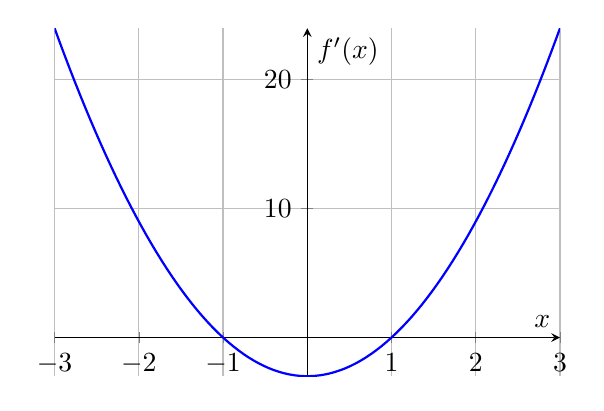
\begin{tikzpicture}
        \begin{axis}[
            axis lines = middle,
            xlabel = \( x \),
            ylabel = \( f'(x) \),
            domain = -3:3,
            samples = 100,
            grid = both,
            width = 8cm,
            height = 6cm
            ]
            \addplot[blue, thick] {3*x^2 - 3};
            \title{Derivative: \( f'(x) = 3x^2 - 3 \)}
        \end{axis}
    \end{tikzpicture}

    \item \( f(x) = \sin(x) \)
    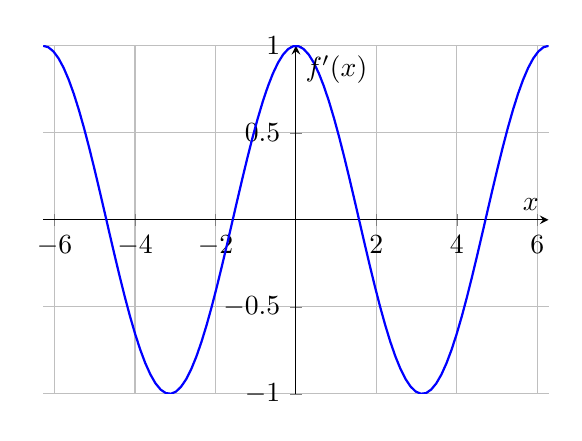
\begin{tikzpicture}
        \begin{axis}[
            axis lines = middle,
            xlabel = \( x \),
            ylabel = \( f'(x) \),
            domain = -2*pi:2*pi,
            samples = 100,
            grid = both,
            width = 8cm,
            height = 6cm
            ]
            \addplot[blue, thick] {cos(deg(x))};
            \title{Derivative: \( f'(x) = \cos(x) \)}
        \end{axis}
    \end{tikzpicture}

    \item \( f(x) = e^x \)
    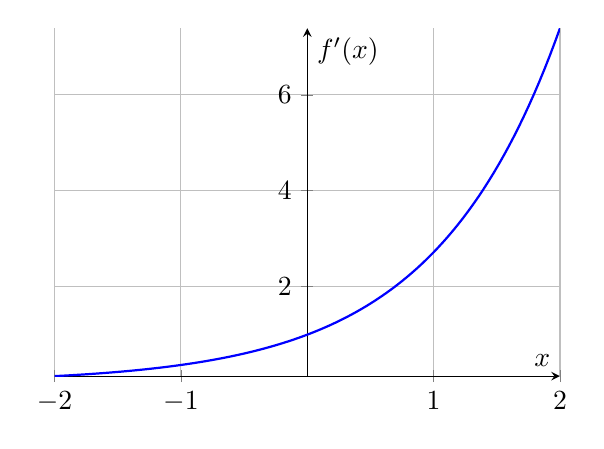
\begin{tikzpicture}
        \begin{axis}[
            axis lines = middle,
            xlabel = \( x \),
            ylabel = \( f'(x) \),
            domain = -2:2,
            samples = 100,
            grid = both,
            width = 8cm,
            height = 6cm
            ]
            \addplot[blue, thick] {exp(x)};
            \title{Derivative: \( f'(x) = e^x \)}
        \end{axis}
    \end{tikzpicture}

    \item \( f(x) = \ln(x) \) for \( x > 0 \)
    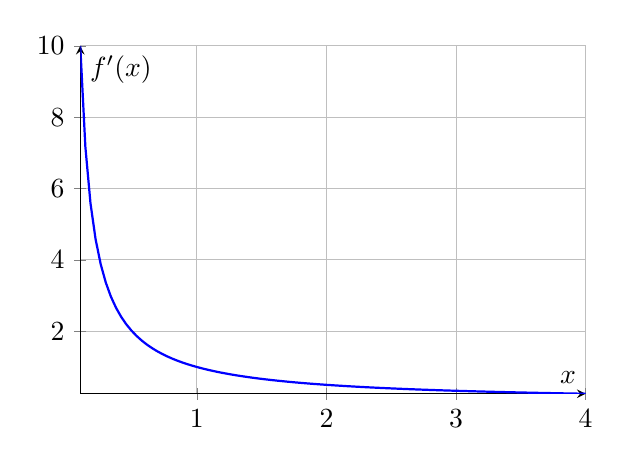
\begin{tikzpicture}
        \begin{axis}[
            axis lines = middle,
            xlabel = \( x \),
            ylabel = \( f'(x) \),
            domain = 0.1:4,
            samples = 100,
            grid = both,
            width = 8cm,
            height = 6cm
            ]
            \addplot[blue, thick] {1/x};
            \title{Derivative: \( f'(x) = \frac{1}{x} \)}
        \end{axis}
    \end{tikzpicture}

    \item \( f(x) = |x| \)
    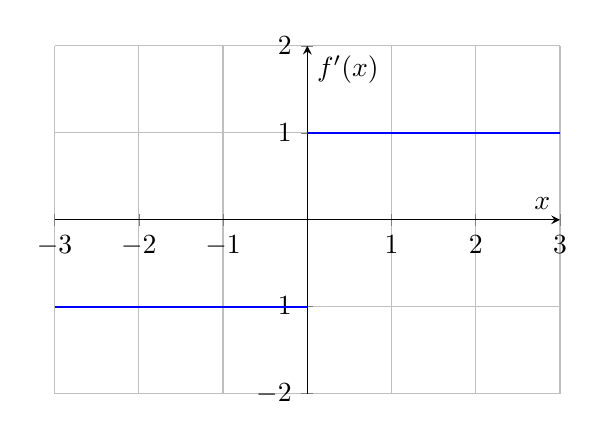
\begin{tikzpicture}
        \begin{axis}[
            axis lines = middle,
            xlabel = \( x \),
            ylabel = \( f'(x) \),
            domain = -3:3,
            samples = 100,
            grid = both,
            width = 8cm,
            height = 6cm,
            ymin = -2, ymax = 2
            ]
            \addplot[blue, thick, domain=-3:0] {-1};
            \addplot[blue, thick, domain=0:3] {1};
            \title{Derivative: \( f'(x) = \pm 1 \)}
        \end{axis}
    \end{tikzpicture}

\end{enumerate}


   



    \item \textbf{Solution to Question 16:}
    Evaluate:
    \[
    \lim_{x \to 0^+} \frac{|x|}{x} = 1 \quad \text{and} \quad \lim_{x \to 0^-} \frac{|x|}{x} = -1
    \]
    Since the limits are not equal, the derivative does not exist at \( x = 0 \).

    \item \textbf{Solution to Question 17:}
    If \( f(x) \) is differentiable at \( x = a \), then it must be continuous at \( x = a \). This is because differentiability implies the existence of a finite limit, which necessitates continuity.

    

    

    \item \textbf{Solution to Question 18:}

    Consider the piecewise function \( f(x) = 
    \begin{cases} 
    x^2 & \text{if } x < 1 \\
    2x & \text{if } x \geq 1 
    \end{cases} \).

    To determine whether \( f(x) \) is differentiable at \( x = 1 \), we need to check if the derivative from the left and right at \( x = 1 \) are equal.

    \textbf{Step 1: Calculate the left-hand derivative.}

    For \( x < 1 \), \( f(x) = x^2 \).

    \[
    f'(x) = \frac{d}{dx} (x^2) = 2x
    \]
    Evaluating at \( x = 1 \):

    \[
    \text{Left-hand derivative at } x = 1: \quad f'_-(1) = 2(1) = 2
    \]

    \textbf{Step 2: Calculate the right-hand derivative.}

    For \( x \geq 1 \), \( f(x) = 2x \).

    \[
    f'(x) = \frac{d}{dx} (2x) = 2
    \]
    Evaluating at \( x = 1 \):

    \[
    \text{Right-hand derivative at } x = 1: \quad f'_+(1) = 2
    \]

    \textbf{Step 3: Conclusion}

    Since the left-hand derivative \( f'_-(1) = 2 \) and the right-hand derivative \( f'_+(1) = 2 \) are equal, the function \( f(x) \) is differentiable at \( x = 1 \).

    \item \textbf{Solution to Question 19:}

    Consider the function \( f(x) = |x - 1| \). To understand why the derivative does not exist at \( x = 1 \), we examine the left-hand and right-hand derivatives.

    \textbf{Step 1: Express the piecewise definition of \( f(x) \).}

    \[
    f(x) = 
    \begin{cases} 
    1 - x & \text{if } x < 1 \\
    x - 1 & \text{if } x \geq 1 
    \end{cases}
    \]

    \textbf{Step 2: Calculate the left-hand derivative.}

    For \( x < 1 \), \( f(x) = 1 - x \).

    \[
    f'(x) = -1
    \]

    \textbf{Step 3: Calculate the right-hand derivative.}

    For \( x \geq 1 \), \( f(x) = x - 1 \).

    \[
    f'(x) = 1
    \]

    \textbf{Step 4: Conclusion}

    The left-hand derivative at \( x = 1 \) is \( -1 \), and the right-hand derivative at \( x = 1 \) is \( 1 \). Since these two derivatives are not equal, the derivative of \( f(x) \) does not exist at \( x = 1 \).

    \item \textbf{Solution to Question 20:}

    Consider the function \( f(x) = x^{1/3} \).

    \begin{enumerate}[label=(\alph*), itemsep=10pt]
        \item \textbf{Find the derivative of the function.}

        To differentiate \( f(x) = x^{1/3} \), we use the power rule:

        \[
        f'(x) = \frac{d}{dx} x^{1/3} = \frac{1}{3}x^{-2/3} = \frac{1}{3} \cdot \frac{1}{x^{2/3}} = \frac{1}{3x^{2/3}}
        \]

        \item \textbf{Discuss the behavior of the derivative near \( x = 0 \) and explain why the tangent line is vertical at \( x = 0 \).}

        As \( x \) approaches 0, \( f'(x) \) becomes:

        \[
        f'(x) = \frac{1}{3x^{2/3}} \quad \text{which becomes infinite as } x \to 0.
        \]

        This means the slope of the tangent line at \( x = 0 \) is infinitely steep, which implies that the tangent line is vertical at \( x = 0 \).
    \end{enumerate}

    \item \textbf{Solution to Question 21:}

    The effectiveness of a drug is modeled by \( E(d) = d(10 - d) \), where \( d \) is the dosage.

    \begin{enumerate}[label=(\alph*), itemsep=10pt]
        \item \textbf{Find the dosage that maximizes the drug's effectiveness.}

        First, we find the derivative of \( E(d) \) to locate the critical points:

        \[
        E'(d) = \frac{d}{dd} \left[ d(10 - d) \right] = 10 - 2d
        \]

        Set the derivative equal to zero to find the critical points:

        \[
        10 - 2d = 0 \quad \Rightarrow \quad d = 5
        \]

        So, the dosage that maximizes the drug's effectiveness is \( d = 5 \).

        \item \textbf{Use the second derivative test to confirm whether this dosage is a maximum.}

        Calculate the second derivative of \( E(d) \):

        \[
        E''(d) = \frac{d}{dd} \left( 10 - 2d \right) = -2
        \]

        Since \( E''(5) = -2 < 0 \), the function is concave down at \( d = 5 \), confirming that \( d = 5 \) is indeed the dosage that maximizes the drug's effectiveness.
    \end{enumerate}

    
\end{enumerate}

    \item \textbf{Solution to Question 22:}
\begin{enumerate}[label=(\alph*), itemsep=10pt]
    \item \textbf{Finding the Critical Points:}
    \begin{itemize}
        \item First, find the derivative of the function \( f(x) = \sqrt{x^2 - 8} \).
        \[
        f(x) = (x^2 - 8)^{1/2}
        \]
        Use the chain rule to differentiate:
        \[
        f'(x) = \frac{1}{2}(x^2 - 8)^{-1/2} \cdot 2x = \frac{x}{\sqrt{x^2 - 8}}
        \]

        \item Set the first derivative equal to zero to find the critical points:
        \[
        \frac{x}{\sqrt{x^2 - 8}} = 0
        \]
        Solving for \( x \):
        \[
        x = 0
        \]

        \item To ensure \( x = 0 \) is in the domain of \( f(x) \), verify that \( x^2 - 8 \geq 0 \):
        \[
        x^2 \geq 8 \quad \text{so} \quad |x| \geq \sqrt{8}
        \]
        Since \( 0 \) is not in this domain, \( x = 0 \) is not a valid critical point.
    \end{itemize}

    \item \textbf{Determining Maximum or Minimum:}
    \begin{itemize}
        \item Since there are no valid critical points within the domain \( |x| \geq \sqrt{8} \), check the behavior at the boundary of the domain:
        \[
        x = \pm \sqrt{8}
        \]
        
        \item Evaluate \( f(x) \) at \( x = \pm \sqrt{8} \):
        \[
        f(\sqrt{8}) = \sqrt{(\sqrt{8})^2 - 8} = \sqrt{8 - 8} = 0
        \]
        \[
        f(-\sqrt{8}) = \sqrt{(-\sqrt{8})^2 - 8} = \sqrt{8 - 8} = 0
        \]
        
        \item Since \( f(x) \to \infty \) as \( |x| \to \infty \), there are no local maxima or minima in the usual sense, but \( f(x) = 0 \) at \( x = \pm \sqrt{8} \) are points of interest.
    \end{itemize}



\end{document}
